\section{应用结果展示}  
%\label{chp:display}
在本节中,我们会对RunDroid运行结果做出相应的展示,并将展现结果和静态分析工具FlowDroid的产出结果进行对比,分析各自的优劣。

我们研究的APK的主体代码如\autoref{fig:code_demo}所示。
在\autoref{fig:code_demo}中,我们声明了有Activity\code{MainActivity},他是应用层的主Activity,该Activity界面主要有3个按钮组成,
方便对应的是斐波拉契数量的计算、启动一个Activity(生命周期相关)以及基于Handler的异步事件。



\begin{figure}[!h]
%	\vspace{0.3in}
	\centering
	\begin{lstlisting}[language=Java]
package cn.mijack.rundroidtest;

public class MainActivity extends Activity implements View.OnClickListener {
	Button button1,button2,button3;
	Handler handler = new Handler() {
		public void handleMessage(Message msg) {
			if (msg.what == 1)   
			      Toast.makeText(MainActivity.this, "handle", Toast.LENGTH_SHORT).show();
		}
	};
	protected void onCreate(Bundle savedInstanceState) {
		super.onCreate(savedInstanceState);
		setContentView(R.layout.activity_main);
		button1 = findViewById(R.id.button1);
		button1.setOnClickListener(this);   	
		// button2、button3进行相同的操作,此处省略
	}
	public void onClick(View view) {
		switch (view.getId()) {
			case R.id.button1:		
			     doHandleButton1();		
			     return;				 	
				// button2、button3进行相同的操作,此处省略
		}
	}
	public void doHandleButton1() {
		int fibonacci = doFibonacci(5);
		Toast.makeText(this, "fibonacci: " + fibonacci, Toast.LENGTH_SHORT).show();
	}
	private int doFibonacci(int i) {
		if (i < 1)			return -1;
		if (i == 1 || i == 2) 		return 1;
		return doFibonacci(i - 1) + doFibonacci(i - 2);
	}
	public void doHandleButton2() {
		Intent intent = new Intent(this, NewActivity.class);
		startActivity(intent);
	}
	public void doHandleButton3() {
		Thread workerThread =new WorkerThread(handler);
		workerThread.start();
	}
}\end{lstlisting}
	\caption{MainActvitiy的代码}
	\label{fig:code_demo}
\end{figure}



\subsection{函数调用图的构建结果展示}

在应用程序运行时,点击按钮button1,应用会计算斐波拉契数列中的第5项,并将这个数以Toast的形式展示给用户。
上述过程中,方法调用同时涉及到普通方法调用、递归函数调用。
RunDroid的动态分析结果如\autoref{fig:rundroid-result-Fibonacci}所示:
每一个红色节点对应的是方法执行,\eat{每一个蓝色节点对应的是系统方法执行,}每一个紫色节点对应是一个对象;
如果对象是方法执行的方法对象,则在图中会有一条边从方法指向该对象,并在边上标识两种之间的关系(蓝色有向边表示参数关系、黄色有向边返回值关系等\footnote{由于所有方法的实例对象都是\code{MainActivity},所以实例关系在图中不做展示});
如果两个方法执行之间存在调用关系,则他们之间会通过从调用发起方指向被调用方的绿色有向边进行连接。

在本案例中,\code{doHandleButton1()}调用了方法\code{doFibonacci()},因此前者有条有向边指向后者;
通过观察虚线框中各节点的关系,我们知道,对于方法\code{doFibonacci()},当参数为5时,对应的结果为5。
FlowDroid的静态分析结果如\autoref{fig:flowdroid-result-Fibonacci}所示。
通过比较\autoref{fig:rundroid-result-Fibonacci}和\autoref{fig:flowdroid-result-Fibonacci},我们可以发现以下有趣的现象:


\begin{figure*}[!ht]
	\centering
	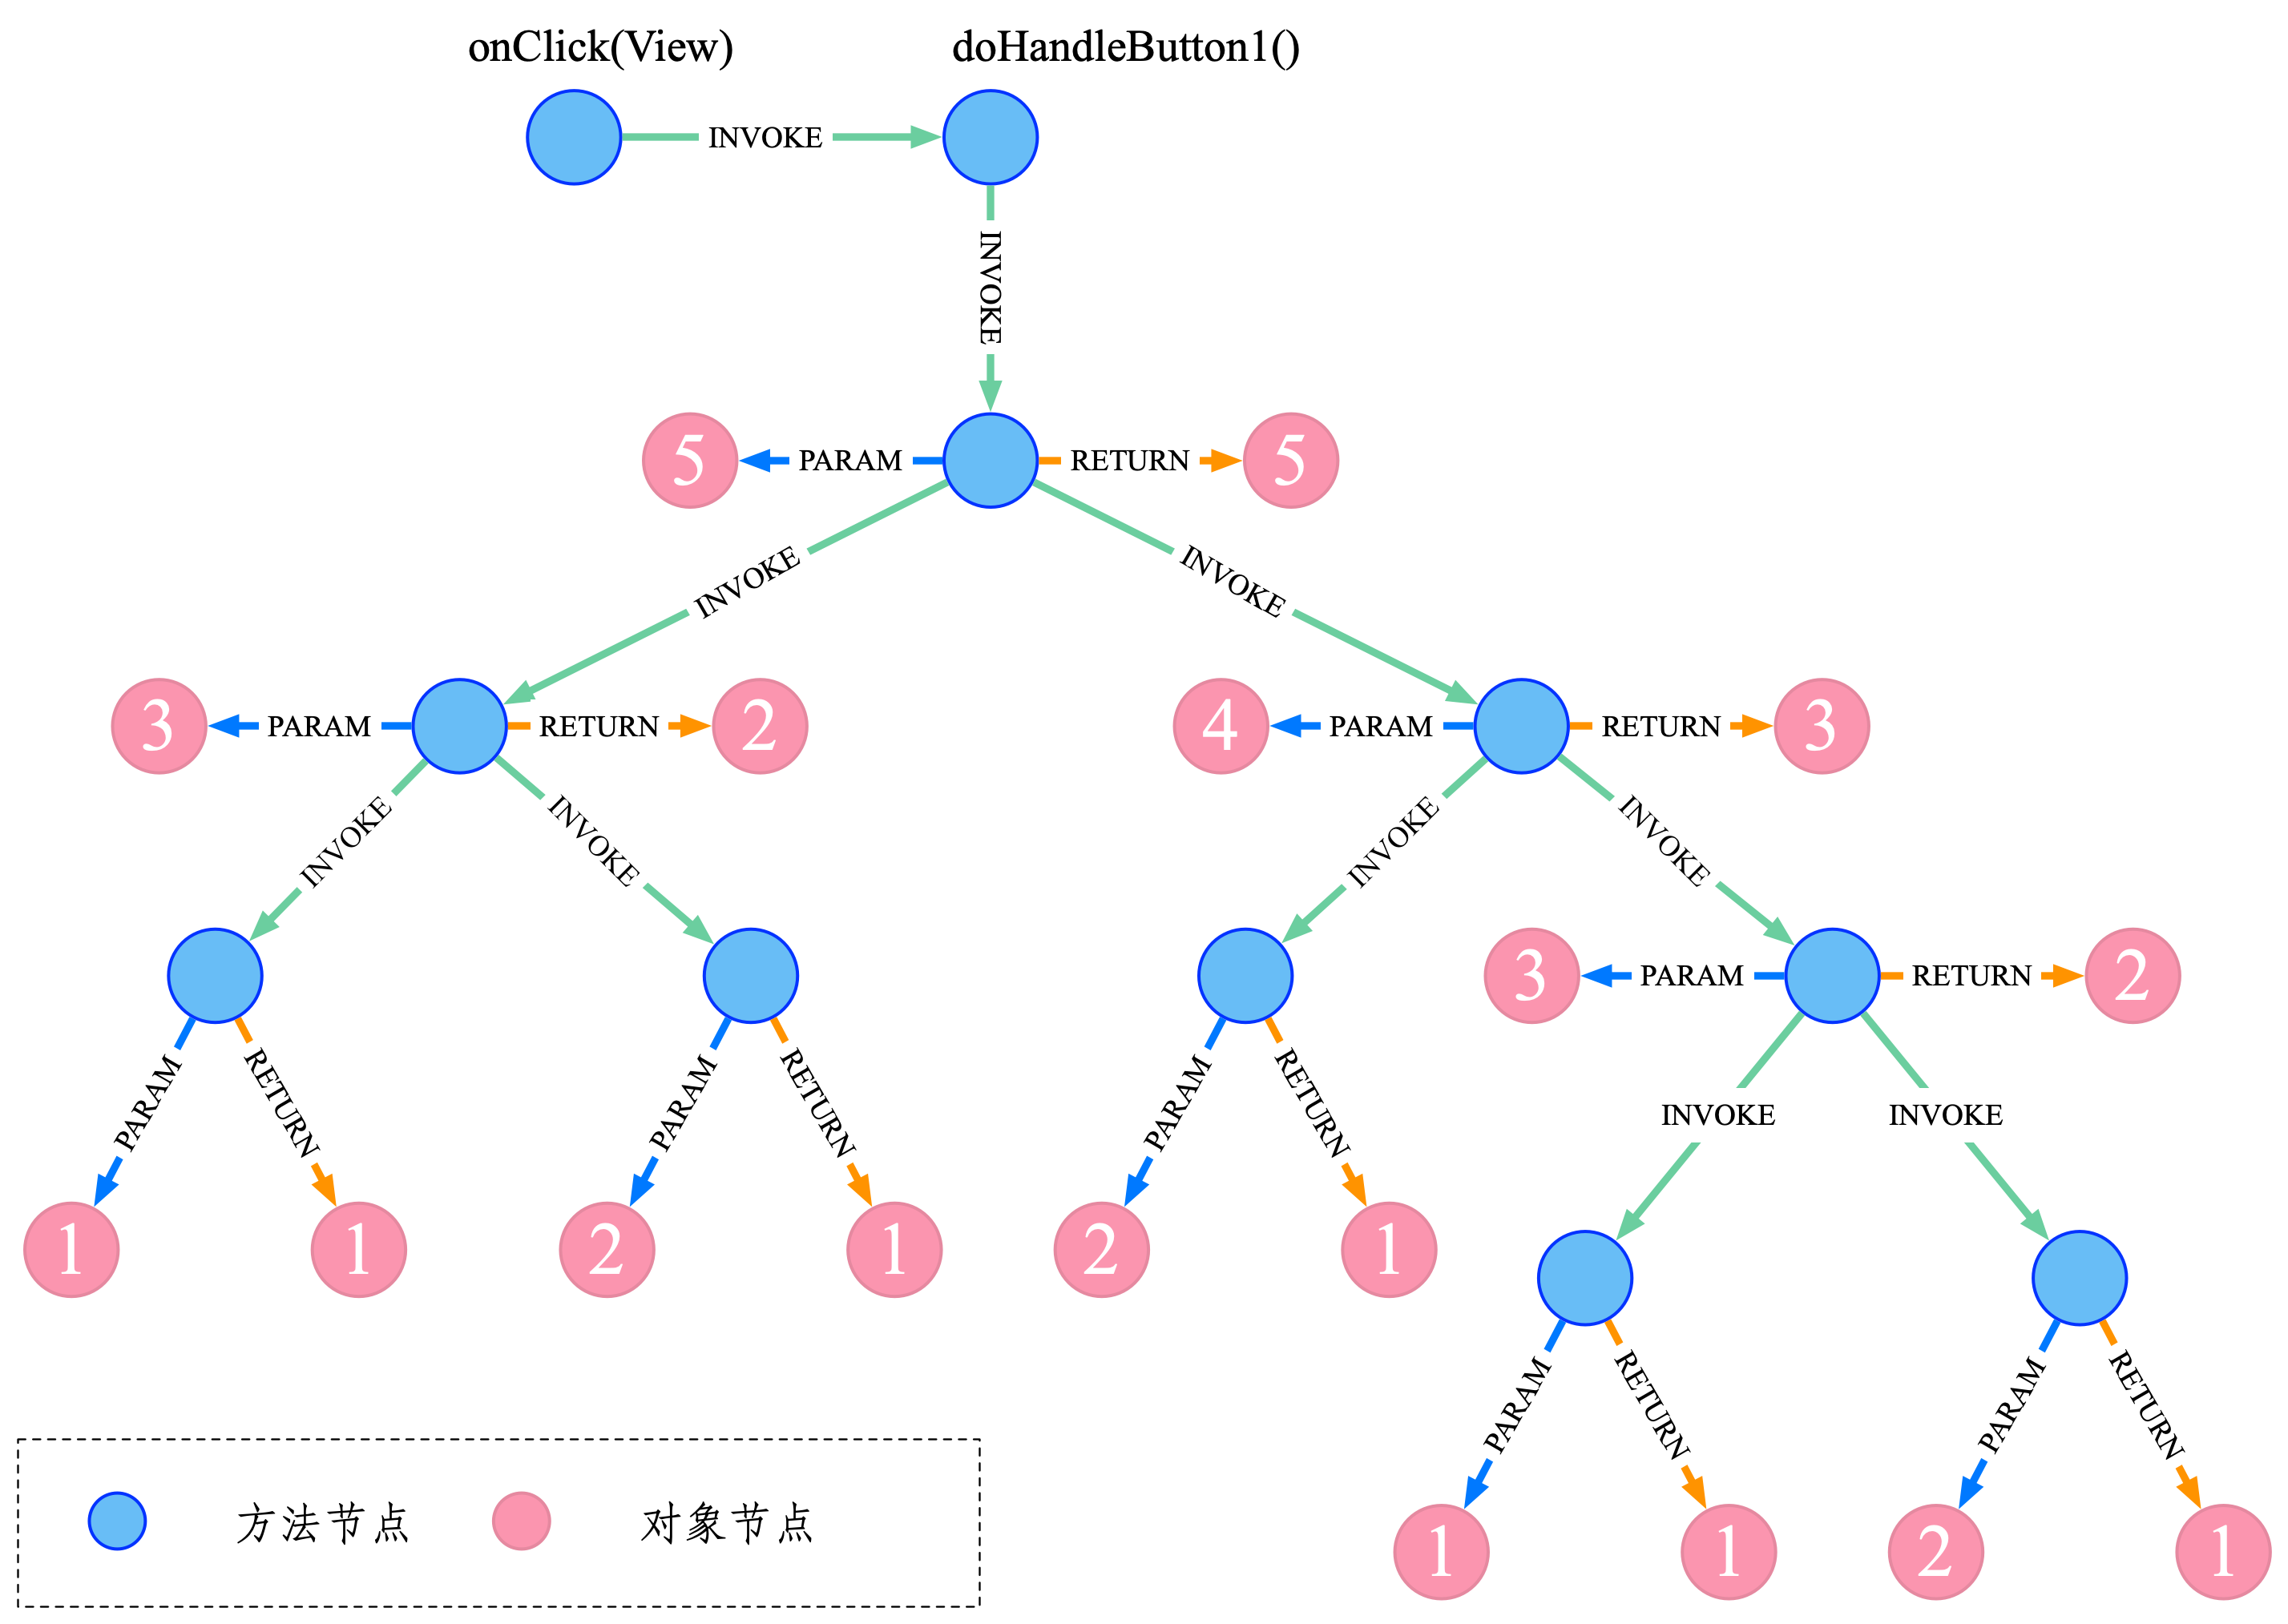
\includegraphics[width=\textwidth]{./Figures/doFibonacci-rundroid.png}
	\caption{斐波拉契数列相关的RunDroid调用图(局部)}
	\label{fig:rundroid-result-Fibonacci}
\end{figure*}

首先,两者在方法\code{doFibonacci()}数量上不同的:RunDroid得到的结果中,方法节点\code{doFibonacci()}共有9个,即在运行过程中,\code{doFibonacci()}被调用了9次。
由于在一个应用中,一个方法的方法签名是唯一的,所以FlowDroid给出的结果中\code{doFibonacci()}只有一个节点。该节点上存在一个指向自己的环,表示这个方法在执行过程中可能出现递归调用的情况。
%另外,静态分析方法(FlowDroid)在分析\code{doFibonacci()}这类方法时,对函数的执行上下文做出准确的判断,进而给出程序准确的运行时行为。
因此,静态分析技术得到的函数调用图往往以方法体本身作为研究的基本单元,而动态分析技术的函数调用图可以细化方法执行之间的关系,反映了程序执行的具体过程。



其次,在运行过程中,斐波拉契数列的计算结果最终以Toast的形式展现在界面上。
但方法\code{Toast.makeText(Context,CharSequence,int)}没有出现在RunDroid的结果中,却出现在FlowDroid给出的结果:
出现这个现象的原因如下:该方法属于系统定义的方法,而运行时拦截器待拦截的方法列表中并未包含该方法,因此运行时未收集到相关的方法执行信息,导致RunDroid无法在调用图中还原相应的函数。
这也反映了RunDroid的不足:关于系统函数的运行时信息的捕获需要提前将相应的方法告知运行时拦截器,生成的调用图才会包括相应的方法。
这使得调用图只包含研究人员关心的方法的执行信息,但也在一定程度上导致部分方法的缺失和调用图的局部不完整。


\begin{figure*}[!ht]
	\centering
	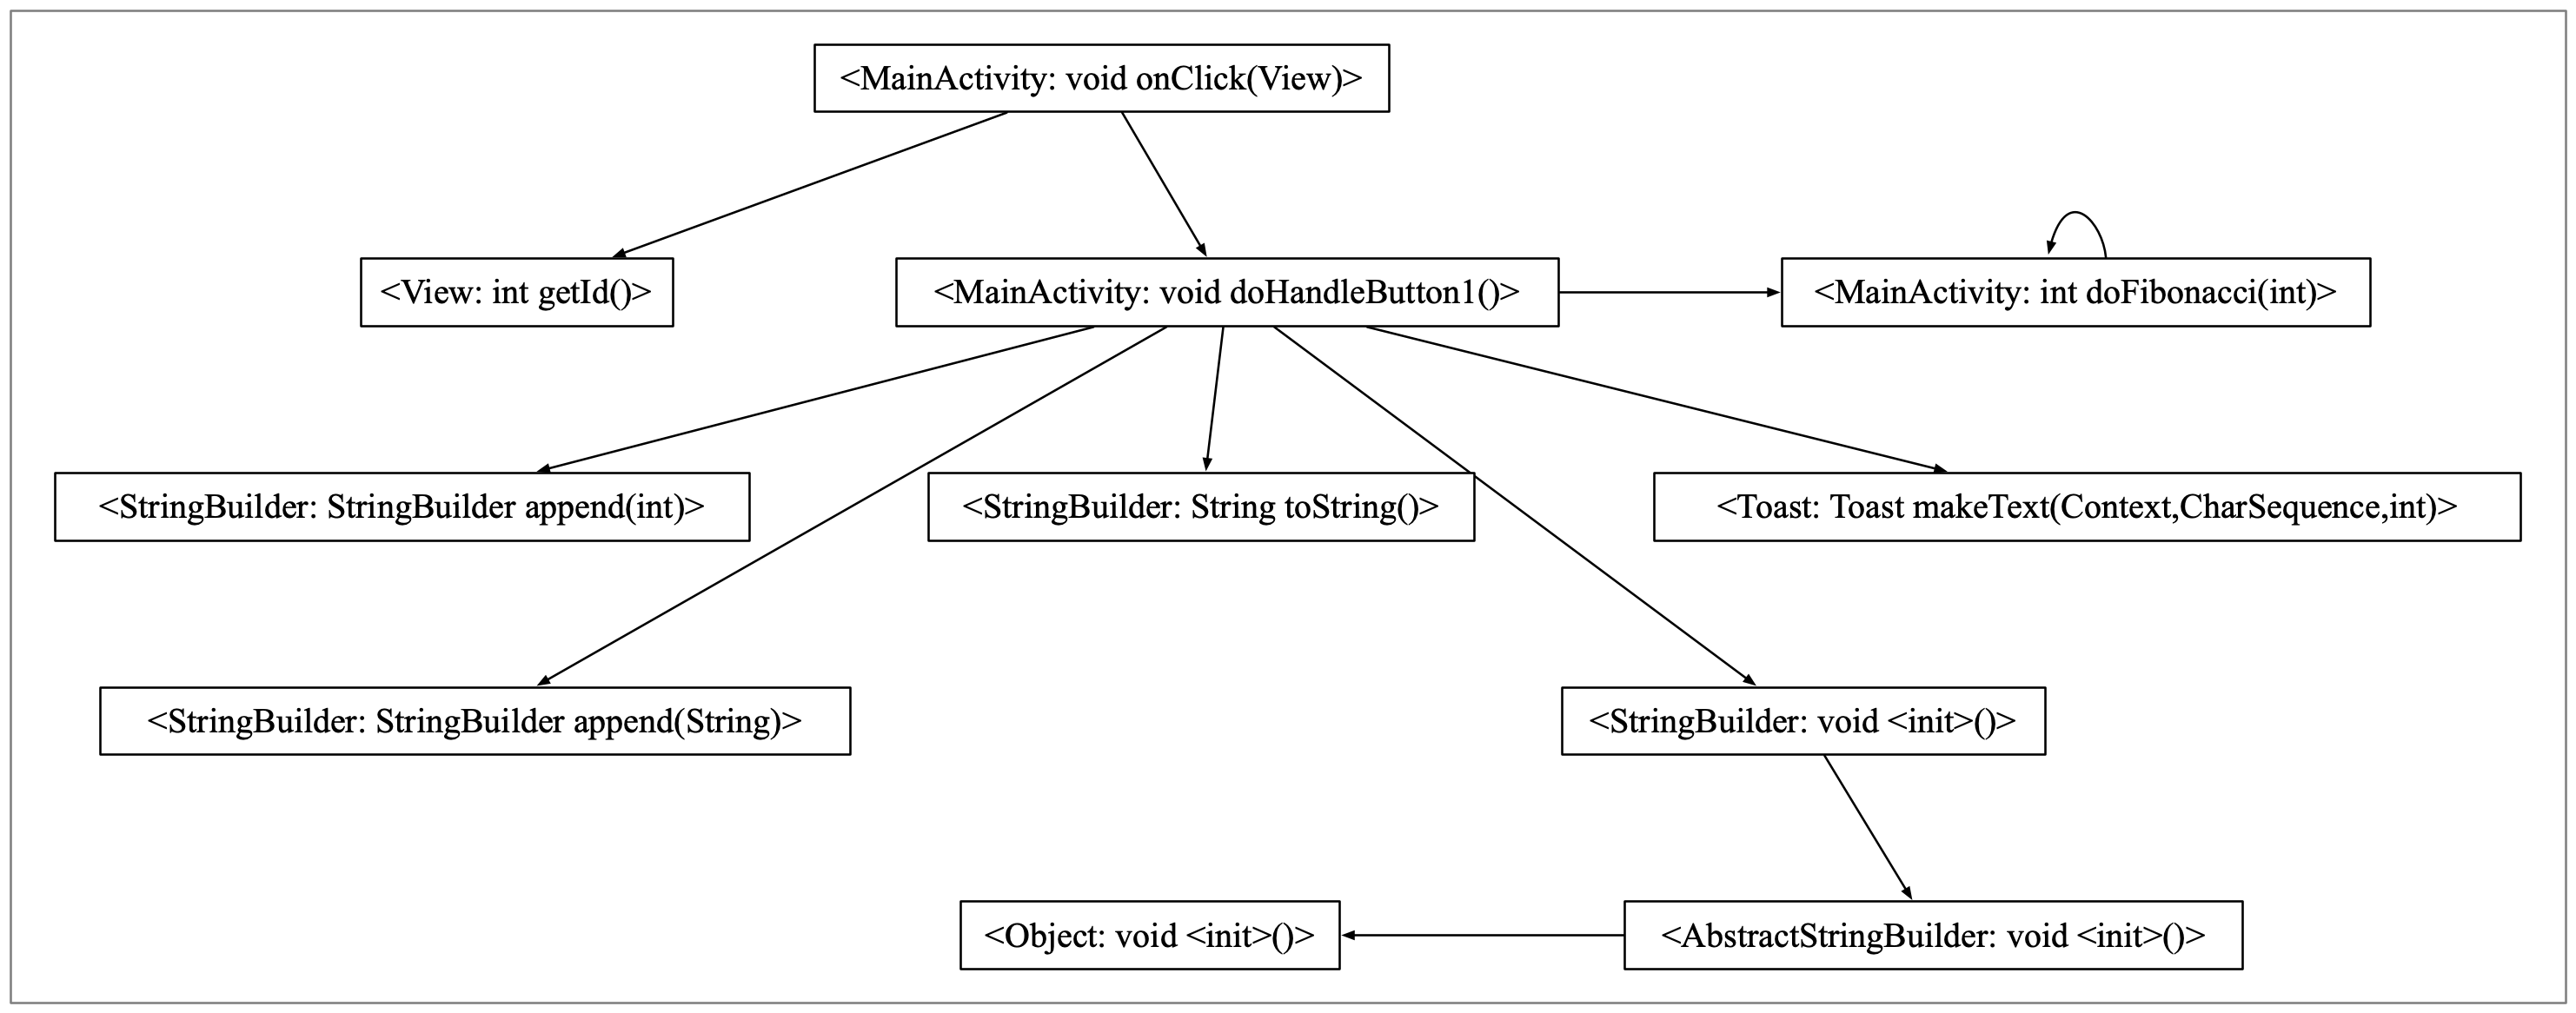
\includegraphics[width=\textwidth]{./Figures/FlowDroid-Fibonacci.png}
	\caption{斐波拉契数列相关的FlowDroid调用图(局部)}
	\label{fig:flowdroid-result-Fibonacci}
\end{figure*}


最后,FlowDroid给出的结果中包括了大量和\code{StringBuilder}相关的方法,而RunDroid的结果并不包括这些方法:
对比源码发现,源程序并未直接使用\code{StringBuilder}。
通过查阅文献\cite{gosling2000java},我们发现出于提高字符串串联性能的考虑,Java编译器可以使用类\code{StringBuilder}等技术通过源代码做适当等价的修改,以避免表达式求值过程中产生过多的字符串数量。
由于上述过程发生在Java程序编译阶段并最后以字节码的形式保存在APK文件中,而FlowDroid从字节码层面对应用进行分析,因此FlowDroid的分析结果会包含该方法。
对于RunDroid,上述方法既在源代码中未出现相关方法定义(无法进行日志代码编织),又不在运行时拦截器的目标方法列表中,所以RunDroid给出的调用图自然也不会包括\code{StringBuilder}相关的方法。



\subsection{Activity 生命周期和事件回调的效果展示}

在本节中,应用运行时,我们将点击按钮button2,在\code{MainActivity}启动另一个\code{NewActivity},对比RunDroid和FlowDroid在Activity生命周期方法的呈现效果。
最终,我们得到的RunDroid的运行结果如\autoref{fig:rundroid-result-lifecycle}所示。
针对Android 组件\code{Activity}的生命周期特性,FlowDroid 进行了针对性的建模,通过构造方法\code{dummyMainMethod()}串联Android Activity的生命周期和UI事件回调,相应的结果如\autoref{fig:flowdroid-result-lifecycle}所示。

\begin{figure*}[ht]
	\centering
	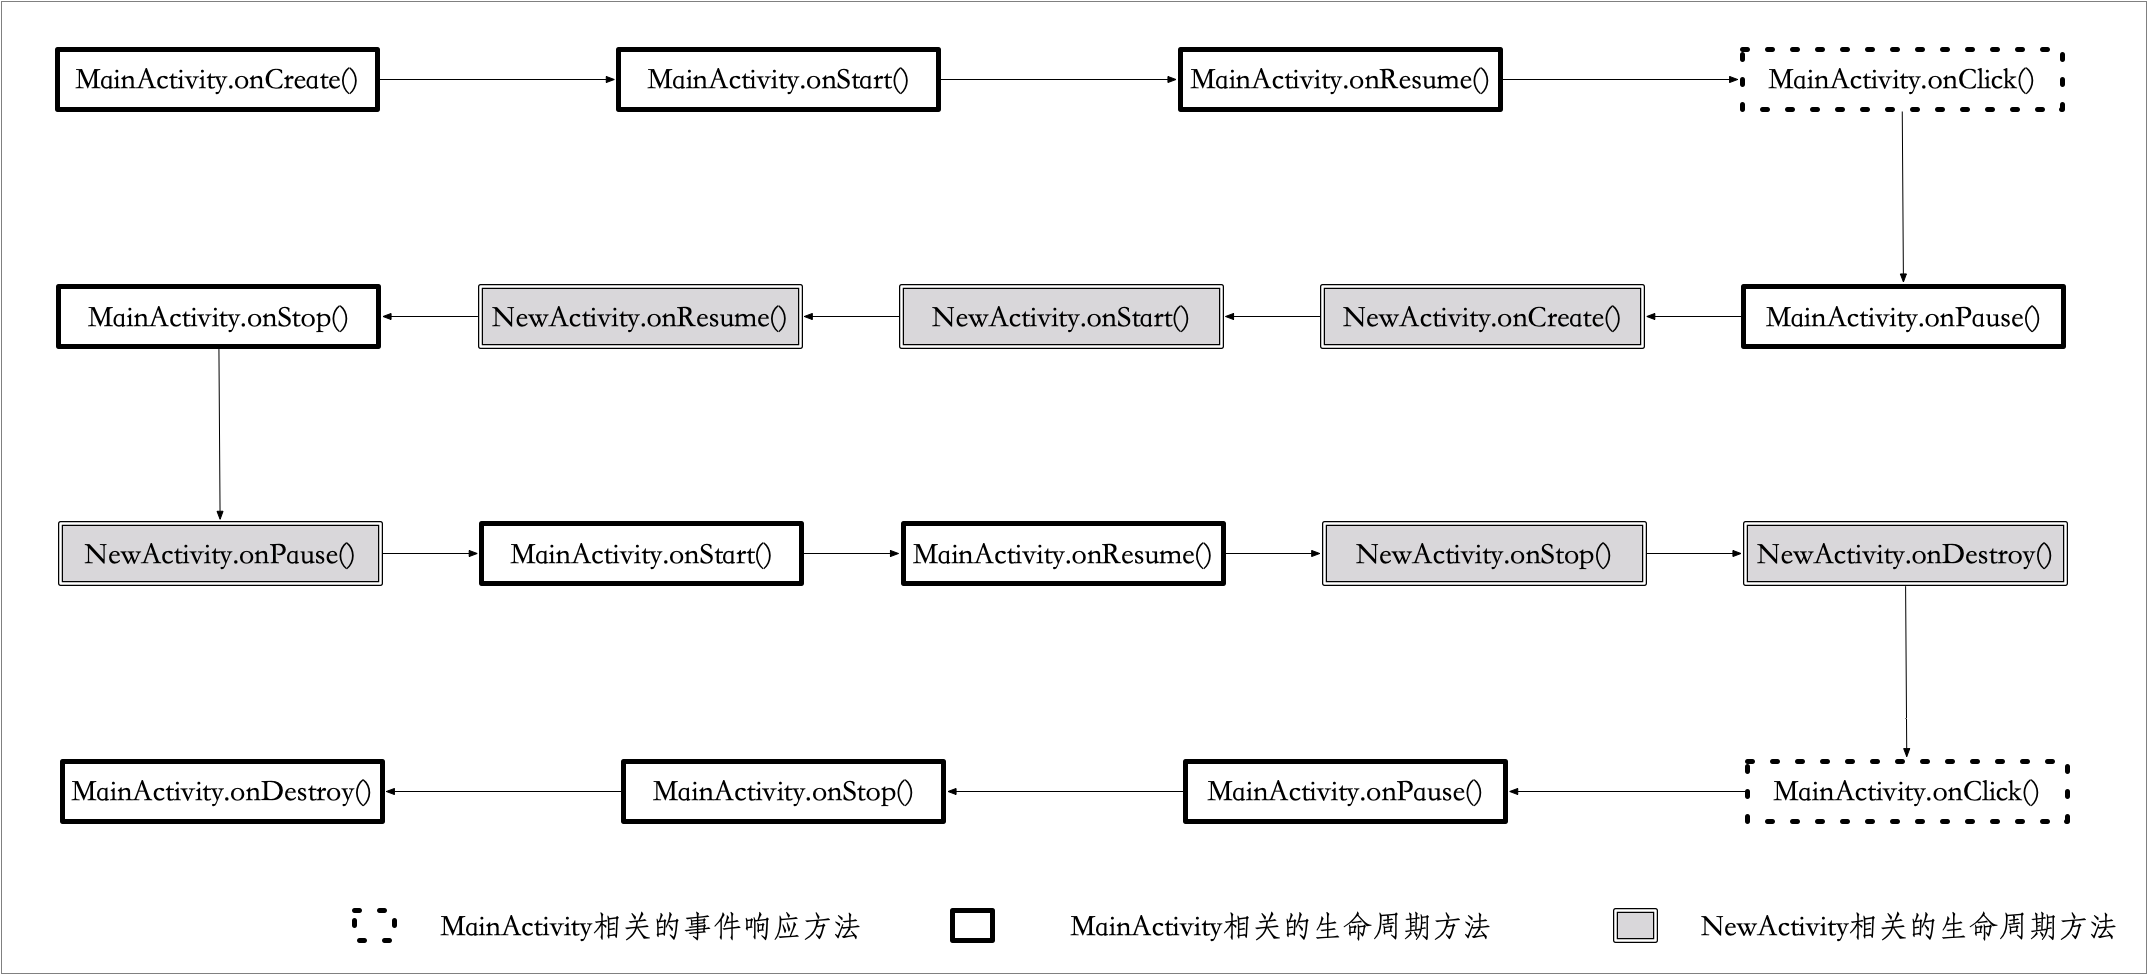
\includegraphics[width=\textwidth]{./Figures/android-lifecycle-rundroid.png}
	\caption{Activity生命周期和事件回调的调用图(局部)}
	\label{fig:rundroid-result-lifecycle}
\end{figure*}

对比\autoref{fig:rundroid-result-lifecycle}和\autoref{fig:flowdroid-result-lifecycle},
我们可以发现RunDroid和FlowDroid在组件生命周期和事件回调上的设计思想上是不同的:
RunDroid可以捕获到组件生命周期方法以及回调事件方法的实际执行,因此,RunDroid对于上述行为的展现主要是按照时间的先后顺序将这些方法节点串联起来,形成完整的事件序列。
而FlowDroid在生成函数\code{dummyMainMethod()}时,会为AndroidManifest.xml文件中定义的每一个Activity单独创建包含生命周期方法和事件回调方法的状态迁移图
(\autoref{fig:flowdroid-result-lifecycle}中的虚线框部分表示每个Activity各自的整体状态迁移,灰色部分为\code{MainActivity}中的UI事件响应方法),
最后将这些Activity的状态迁移串联起来,并将Action为\code{android.intent.action.MAIN}并且category为\code{android.intent.category.LAUNCHER}的Activity组件作为结果的默认启动的Activity,最终形成方法\code{dummyMainMethod()}。


\begin{figure*}[ht]
	\centering
	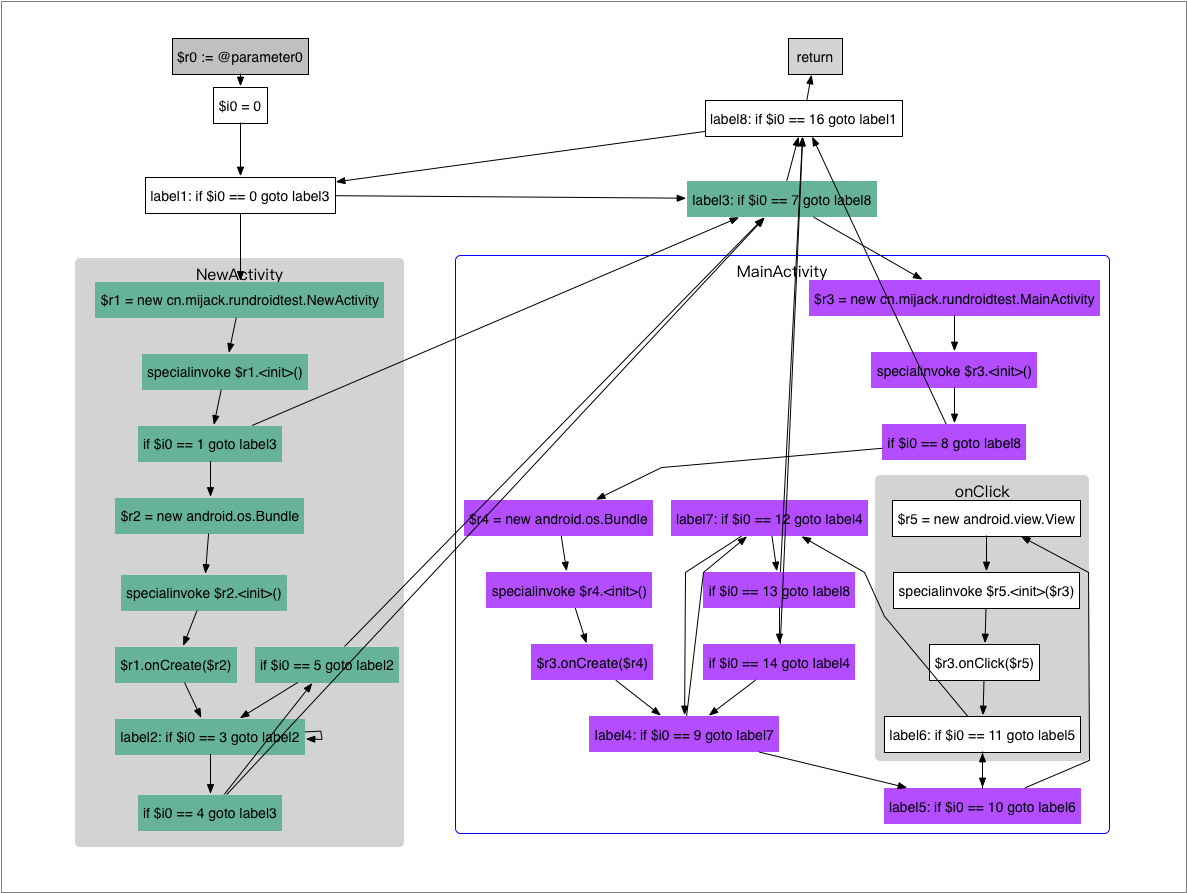
\includegraphics[width=\textwidth]{./Figures/flowdroid-dummyMainMethod.png}
	\caption{FlowDroid生成的函数dummyMainMethod()的调用图}
	\label{fig:flowdroid-result-lifecycle}
\end{figure*}

在结果展现上,RunDroid倾向于展现所有和Activity生命周期相关的方法。
例如,虽然开发人员在源代码中没有定义\code{onResume()}等方法,但在运行过程中,\code{MainActivity}的父类方法\code{onResume()}被调用了,便会出现在RunDroid的结果中。
而FlowDroid在这点上的处理方式恰恰相反:FlowDroid认为一个父类方法未被重写,则该方法运行行为表现保持一致性,FlowDroid并不会在结果中展示父类Activity未重载的生命周期方法。



另外,我们发现在应用从\code{MainActivity}切换到\code{NewActivity}过程中,
对应的生命周期变化为\code{MainActivity.onPause()} $\to$\code{NewActivity.onCreate()}$\to$\code{NewActivity.onStart()}$\to$\code{NewActivity.onResume()}$\to$ \code{MainActivity.onStop()},
\code{MainActivity}和\code{NewActivity}的生命周期方法是交替出现的,
并不是\code{MainActivity}的生命周期方法全部执行完毕后才执行\code{NewActivity}的生命周期方法。
而FlowDroid给出的结果将\code{MainActivty}和\code{NewActivity}分开处理,因此得到的结果属于后面一种情况。
相比FlowDroid,RunDroid的运行结果是程序运行时的直接反映,更适合反映应用的状态变化。


\subsection{多线程触发关系效果展示}

多线程开发是Android开发中经常涉及的开发要求。
为此,针对这一场景,我们进行了相关的测试。
在本节,我们将点击按钮button3,获取\code{doHandleButton3()}相关的调用图情况。
经过实验,RunDroid和FlowDroid的运行结果分别如\autoref{fig:rundroid-result-handler}、\autoref{fig:flowdroid-result-handler}所示。
两幅图在以下节点上存在不同:





\begin{figure*}[ht]
	\centering
	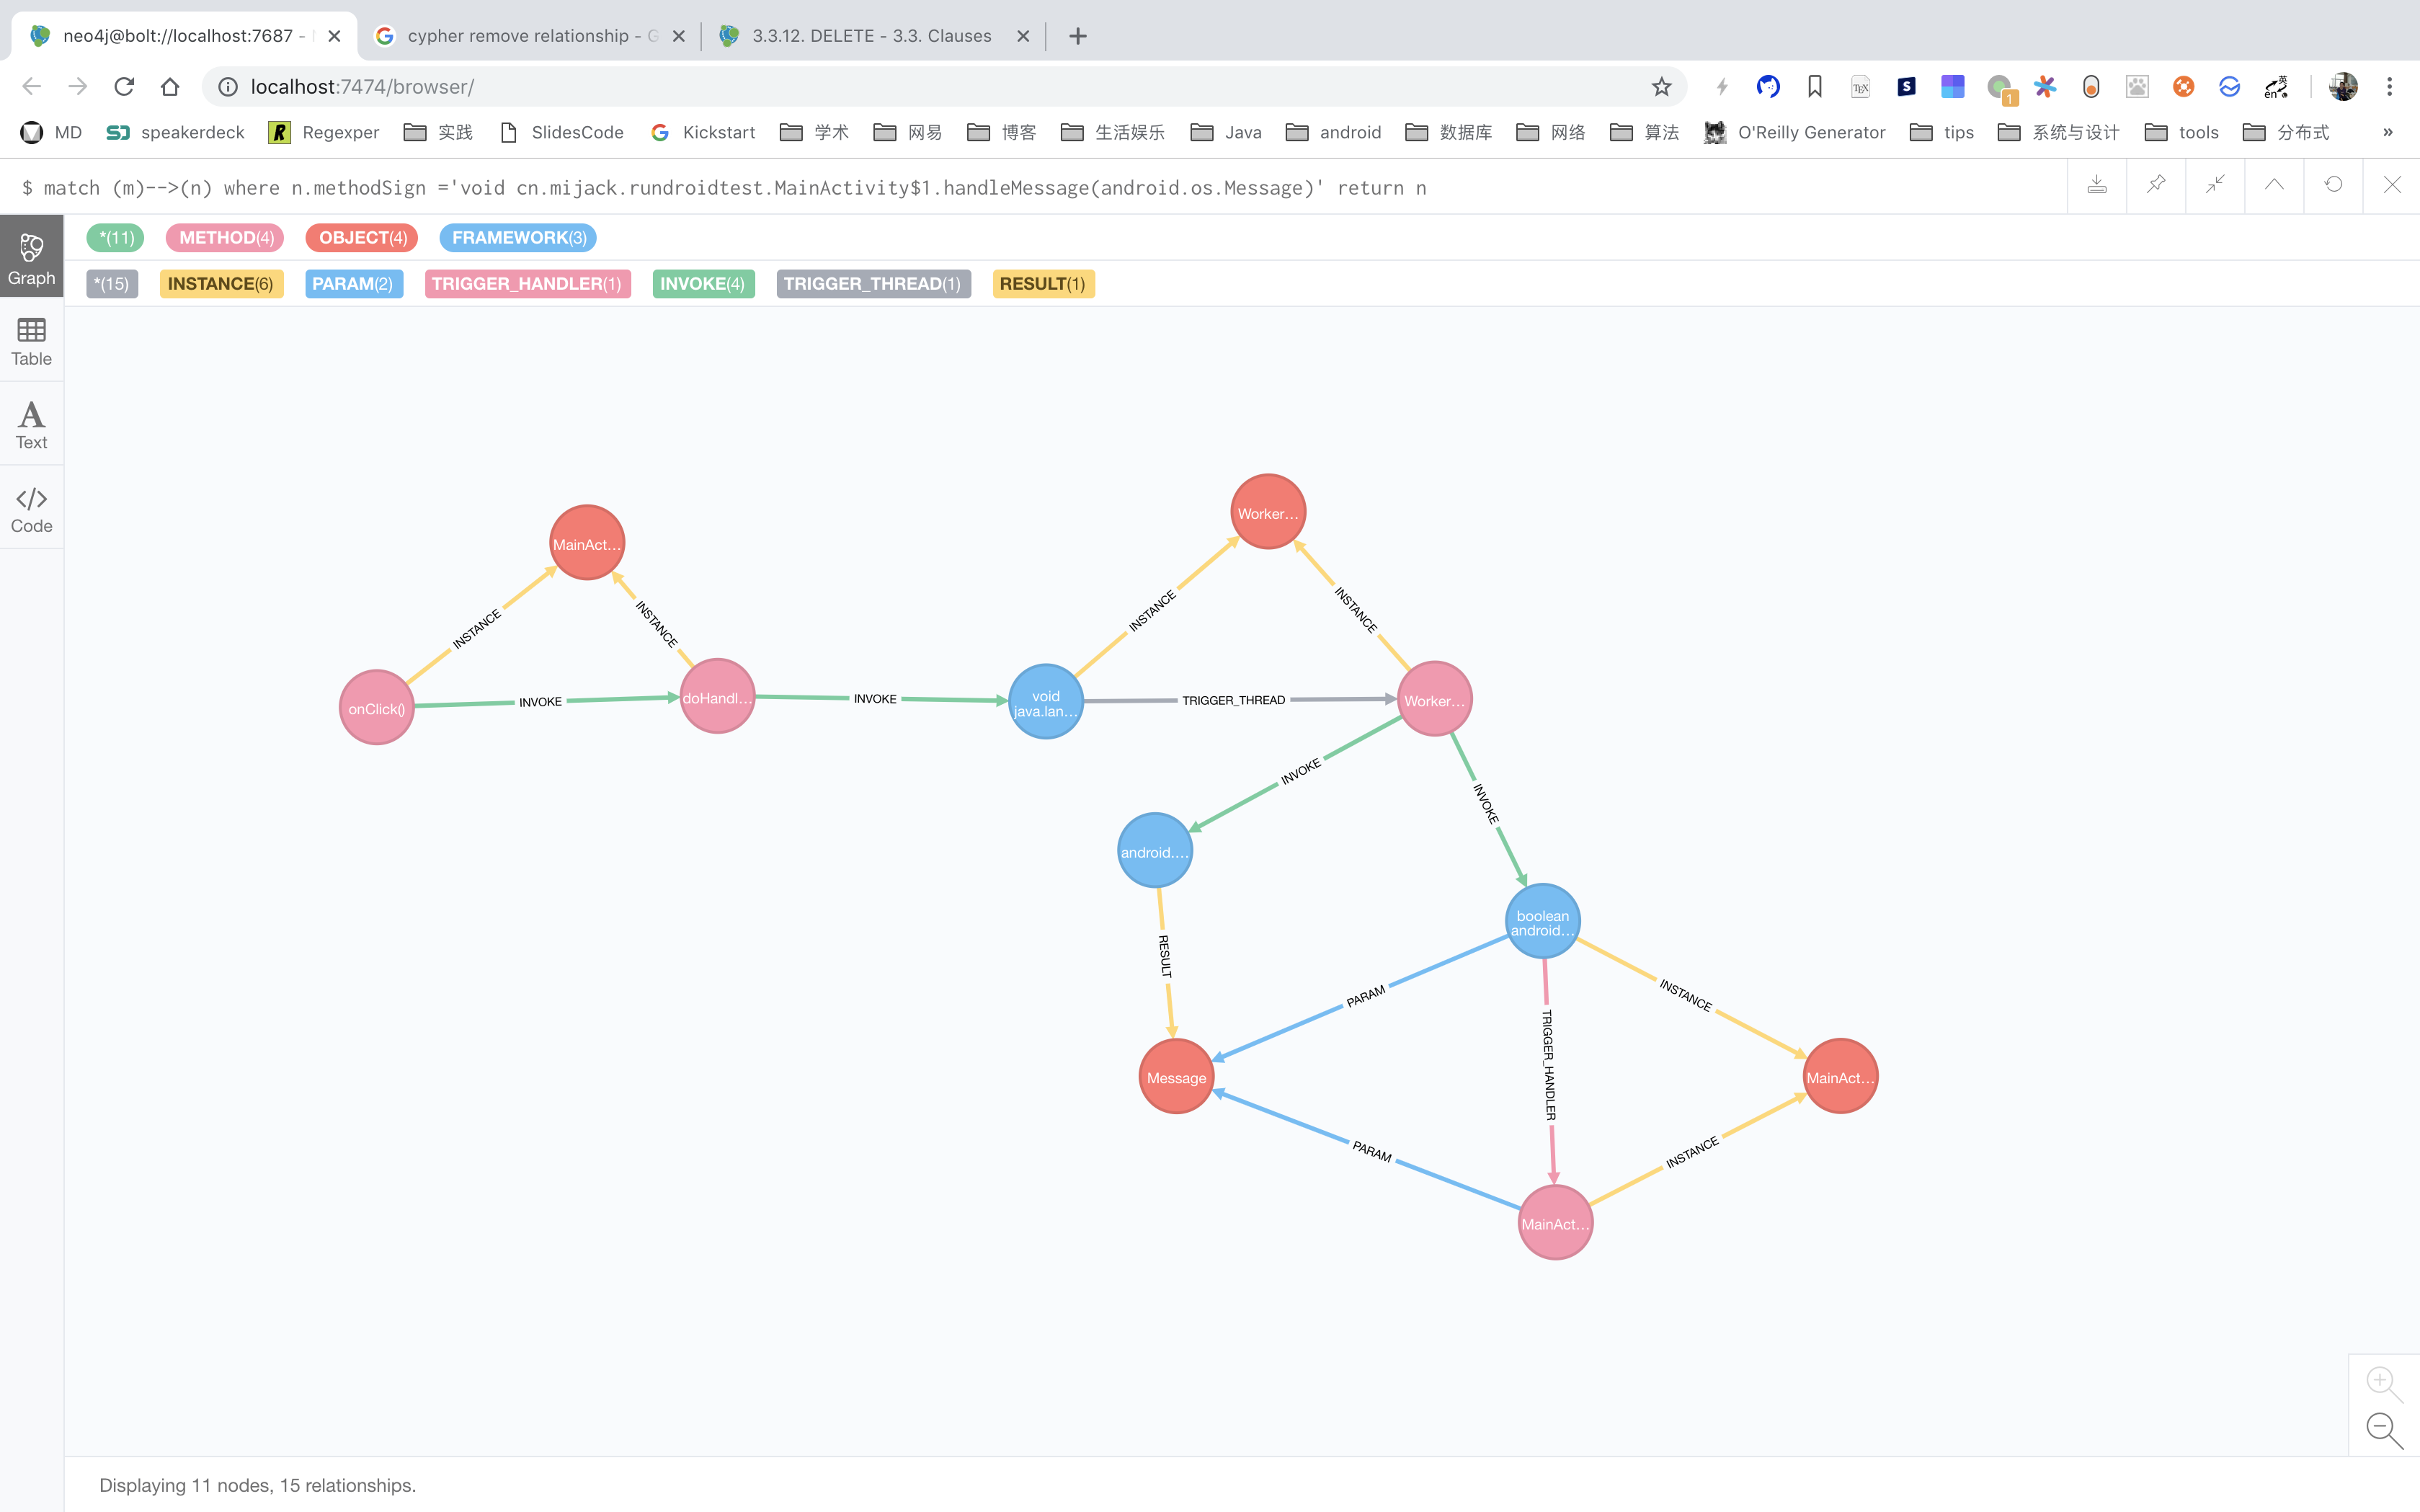
\includegraphics[width=\textwidth]{./Figures/android-handler-rundroid.png}
	\caption{多线程触发关系相关的调用图(局部)}
	\label{fig:rundroid-result-handler}
\end{figure*}






\point{Java API多线程的触发方式}

RunDroid在方法\code{Thread.start()}和方法\code{WorkerThread.run()}之间添加了一条有向边。
这条有向边从前者指向后者,表示方法\code{Thread.start()}的执行触发了方法\code{WorkerThread.run()}的执行,边上标识着触发原因(通过Thread方式触发,Thread)。
FlowDroid对方法\code{doHandleButton3()}进行推算出\autoref{fig:code_demo}第42行中的变量$workerThread$类型为\code{WorkerThread}。
同时,FlowDroid可以推算出方法\code{Thread.start()}的执行会导致方法\code{WorkerThread.run()}的执行。
在FlowDroid的设计者看来,方法\code{Thread.start()}可以替换成方法\code{WorkerThread.run()}。
因此,FlowDroid的结果中,方法\code{doHandleButton3()}和\code{WorkerThread.run()}之间存在调用边。
这条有向边并不是像RunDroid从\code{Thread.start()}出发。
虽然RunDroid和FlowDroid都可以在函数调用图表现Java API多线程的触发方式,但相比之下,RunDroid的呈现方式更为全面严谨,比FlowDroid更符合程序的运行过程。
当方法\code{Thread.start()}和\code{WorkerThread.run()}同时在同一个函数中被调用,FlowDroid在调用图上无法将这两个方法间的调用关系和触发关系区分开。
而RunDroid针对性地标识了函数间的关系是普通调用关系还是基于线程的触发关系,所以不会在方法关系展现上遇到类似的问题。

\begin{figure*}[ht]
	\centering
	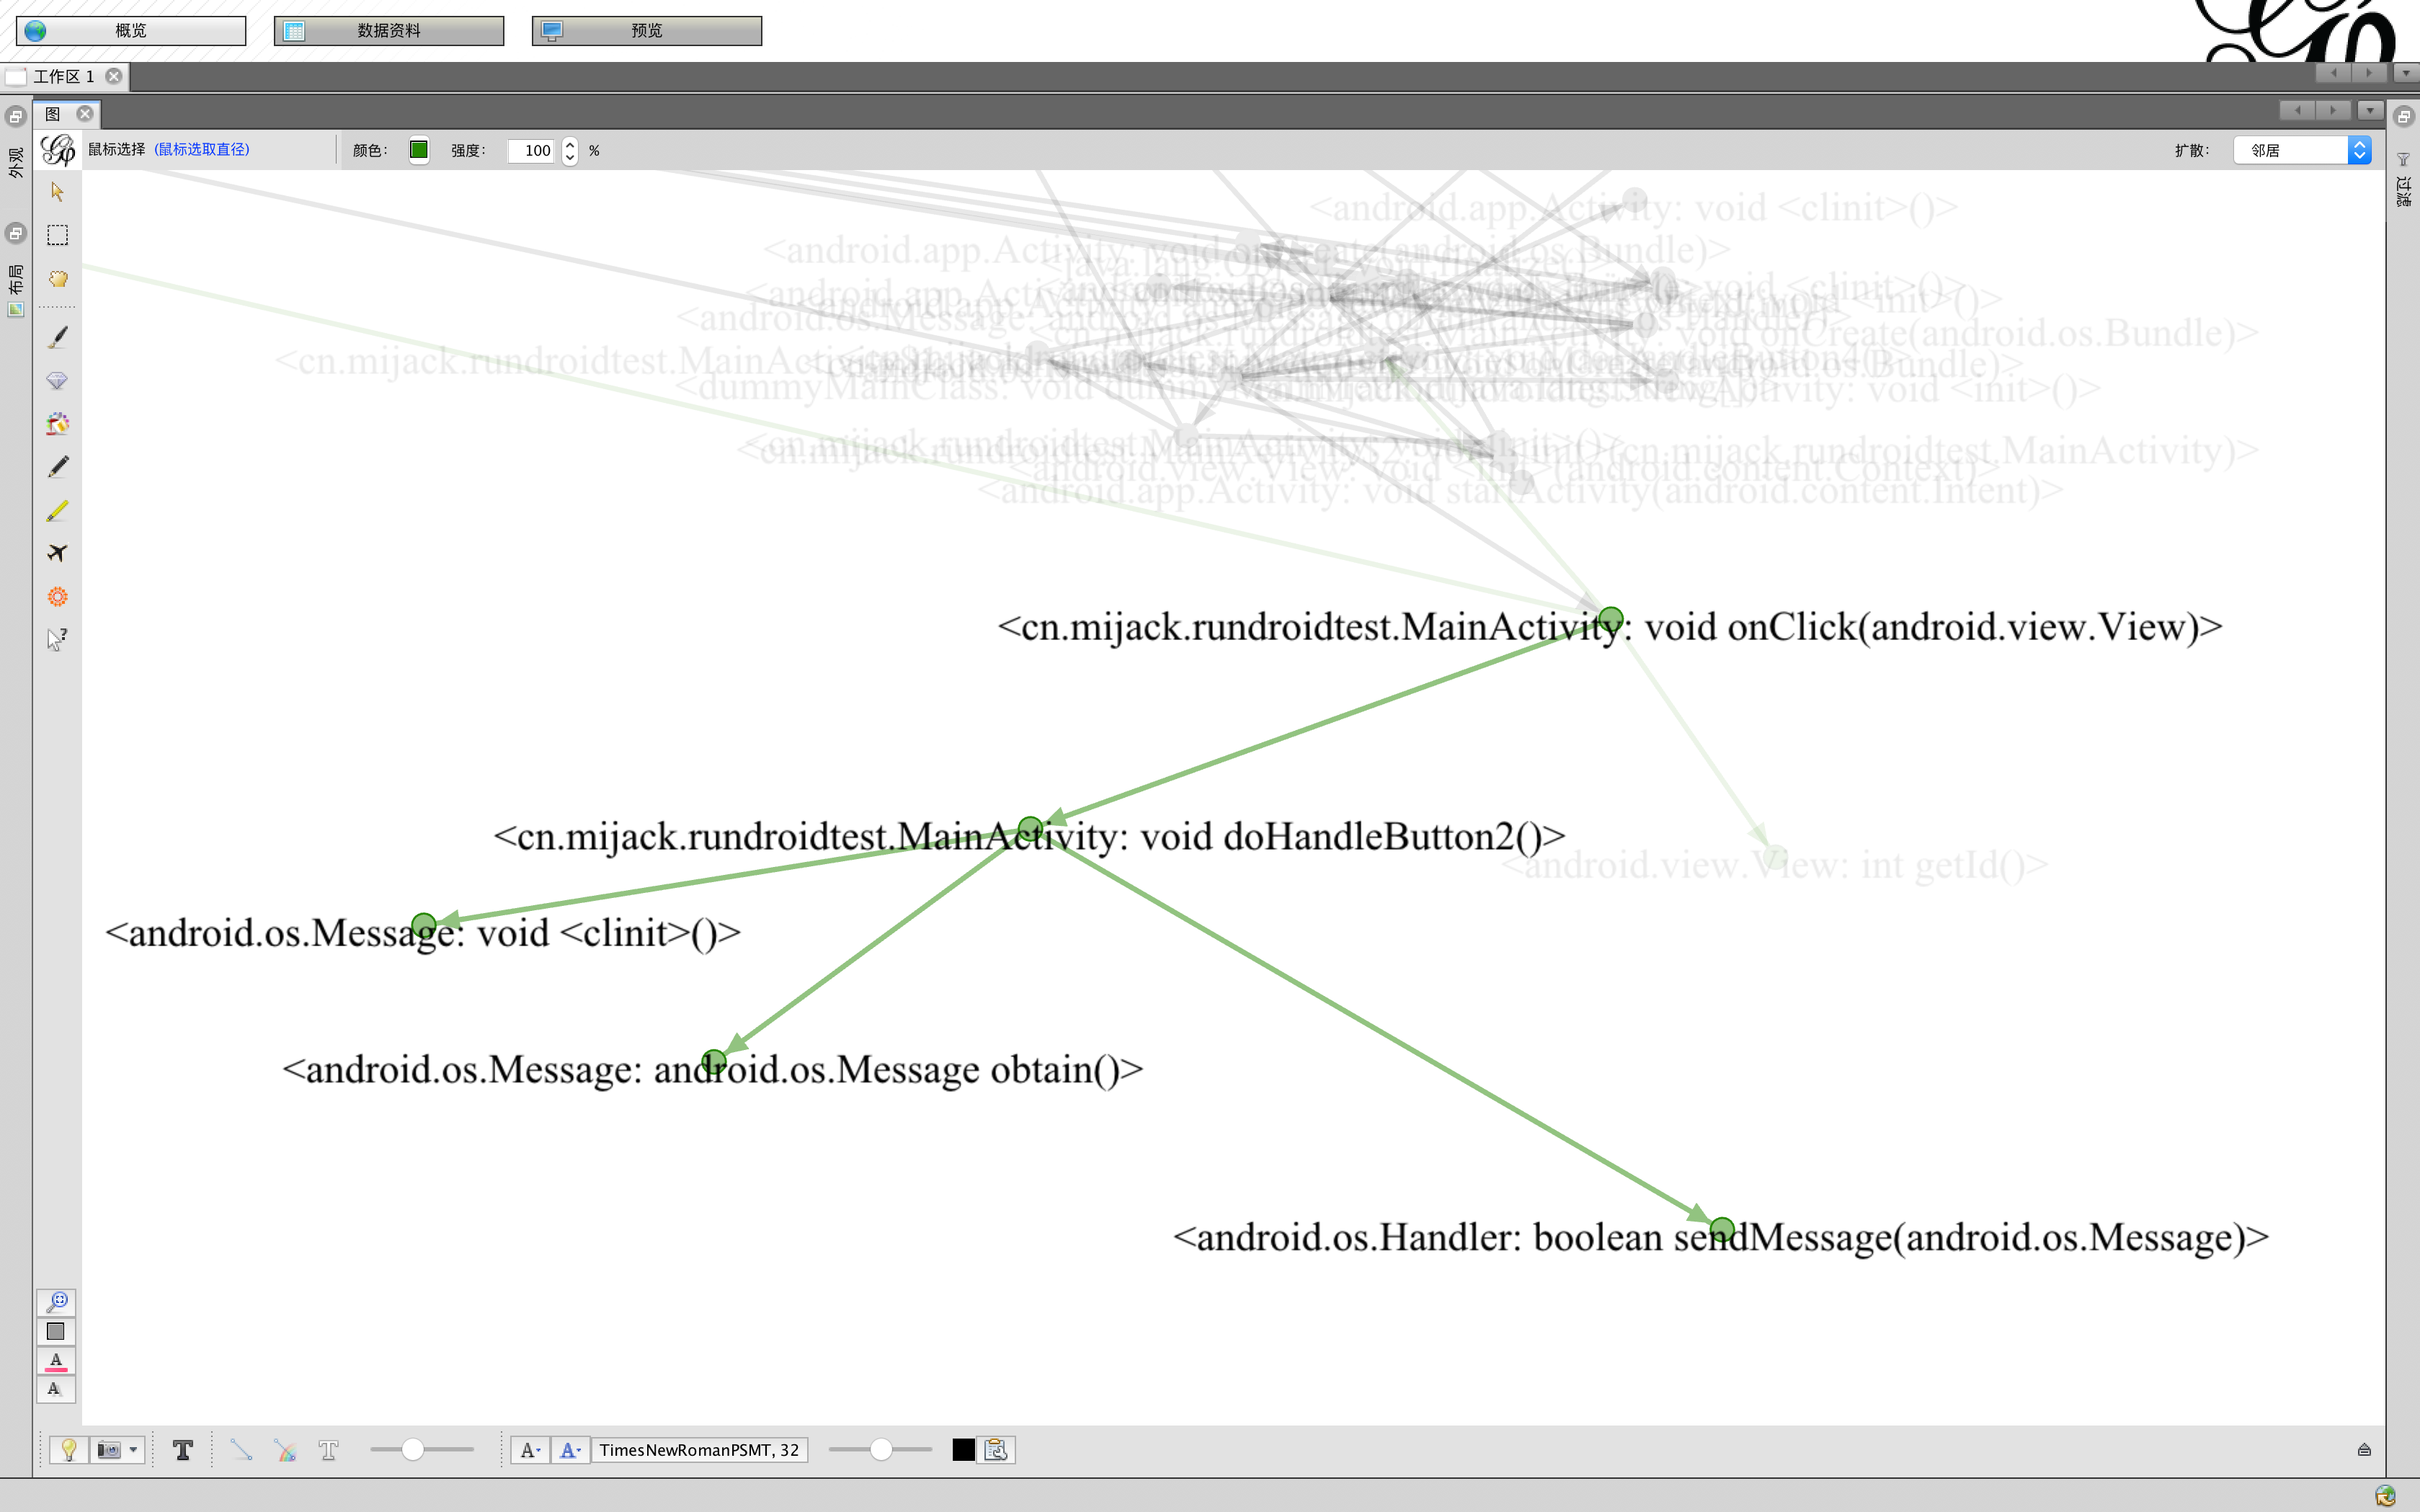
\includegraphics[width=\textwidth]{./Figures/FlowDroid-handler.png}
	\caption{多线程触发关系-FlowDroid生成的调用图(局部)}
	\label{fig:flowdroid-result-handler}
\end{figure*}

\point{基于Handler的多线程触发方式}

在WorkerThread的方法run()中,我们通过Handler进行了异步UI操作,触发了方法\code{MainActivity\$1.handleMessage(Message)}的执行。
在构建拓展调用图过程中,RunDroid充分挖掘了这些方法和对应的方法对象的关联关系,进而补全方法\code{Handler.sendMessage()}和\code{MainActivity\$1.handleMessage(Message)}之间的触发关系。
因此,在RunDroid展示的结果中,上述两个方法之间存在一个从前者指向后者的有向边,边上标识着相应的触发原因(通过Handler方式触发,Handler)\footnote{由于我们定义的Handler是MainActivity的匿名内部类,因此编译后的类名为\code{MainActivity\$1}。}。
但是,FlowDroid分析相关代码时,由于缺少运行时上下文信息,无法分析出\code{WorkerThread.run()}中handler的具体类型,因此无法将这两个方法连接起来。




\point{静态方法的使用}


另外,在FlowDroid给出的结果中,我们发现方法\code{doHandleButton3()}还调用了类\code{Message}的类初始化方法\code{<clinit>()}。
原因是方法\code{doHandleButton3()}调用类\code{Message}的静态方法\code{obtain()},因此可能需要进行类的初始化。
由于在程序运行过中,方法\code{doHandleButton3()}在执行方法\code{Message.obtain()}前,类\code{Message}已经完成了类的初始化,方法\code{Message.<clinit>()}并没有被调用。
因此RunDroid的结果中显示上述两个方法不存在调用关系。
这从一个侧面方面反映出FlowDroid分析的结果和动态运行的过程可能存在一定的偏差。





\section{实验效果评估}

相比其他分析技术,RunDroid最为重要的创新点为在函数调用图中展示函数触发关系(例如多线程相关的触发关系)。
为了验证函数触发关系在Android程序运行过程中的普遍性,我们从开源社区F-Droid\cite{FDroidFr21:online}中随机抽取了9个应用,并针对挑选不同的使用场景进行测试。
我们利用RunDroid构建各应用运行执行情况的函数调用图,统计调用图中的出现函数触发关系数量,结果如\autoref{table:app_results}所示。
我们对表格中的数据逐个进行人工确认,发现实验数据不存在错误。
\todo{从\autoref{table:app_results}中,我们发现对大部分使用场景,应用程序执行过程对应的函数调用图均存在函数触发关系,只是在数量上存在差异。}
由此,我们可以看出函数触发关系在Android应用中的普遍性,也从一个角度验证了第\ref{chp:background}章提到的Android特性:Android应用中存在部分逻辑实现依赖于回调函数和多线程通信。

\begin{table*}[!ht]
	\centering
	{
		\caption{各应用运行过程中的涉及函数触发关系数量}
		\label{table:app_results}
		\begin{tabular}{ |c |c|c|c|c|c|}
			\hline
			应用 &用户方法&系统方法&函数调用关系&函数触发关系\\ 
		%	\cline{5-7}	
		%	~ & ~ & ~  & ~ &\multirow{2}*{ Ui事件}& \multirow{2}*{Thread相关}& Handler           \\ 				
		%	 ~ & ~&~ & ~ & ~         & ~                   & 过滤后/过滤前\\ 				
			\hline
		%	1 &   & 19 & 27(118)& 21 & 3& 1& 1/114& ~ \\ 	
		本章示例             & 19     & 27(700)     & 21                &5(119) \\ 				
			\hline			
			AnyMemo & 1021 & 322(2731) & 1105(3487)& 38(428) \\ 				
			\hline	
			archwiki-viewer & 3699 & 3504 & 310(3342)& 680(21332) \\ 				
			\hline	
			chanu & 1086& 353(3917) & 397(4817)& 34(43440) \\ 				
			\hline	
			Microphone & 31 & 230(1531) & 161(1334)&31 (271)\\ 				
			\hline	
			osmtracker-android & 997& 328(2483) & 1162(2453)& 3(368) \\ 				
			\hline	
			Quran For My Android & 156 & 204(3930) & (3831)&  35(664) \\ 				
			\hline	
			ReGeX & 1415 &95 (987) & 1323(2311)& 39(170)\\ 				
			\hline	
			screenrecorder& 1301 & 320(3278) &879 (4539)& 10(24869)\\ 				
			\hline	
			upm-android & 118& 337( 3097)& 355(2918)&  25(486) \\ 		
			\hline
		\end{tabular}
	}
\end{table*}


\eat{
	
	\begin{table*}[!ht]
		\centering
		{
			\scriptsize
			\caption{各应用运行过程中的涉及函数触发关系数量}

			\begin{tabular}{ |c |c|c|c|c|c|c|c|}
				\hline
				\multirow{3}*{应用 }& \multirow{3}*{用户方法 }  & \multirow{3}*{系统方法} &\multirow{3}{2cm}{\centering 函数调用关系}& \multicolumn{3}{c|}{函数触发关系} \\ 
				\cline{5-7}	
				~ & ~ & ~  & ~ &\multirow{2}*{ Ui事件}& \multirow{2}*{Thread相关}& Handler           \\ 				
				~ & ~&~ & ~ & ~         & ~                   & 过滤后/过滤前\\ 				
				\hline
				%	1 &   & 19 & 27(118)& 21 & 3& 1& 1/114& ~ \\ 	
				本章示例             & 19     & 27(700)     & 21                & 3&1&1(114) \\ 				
				\hline			
				AnyMemo & 1021 & 322(2731) & 1105(3487)& 3& 0& 35(425) \\ 				
				\hline	
				archwiki-viewer & 3699 & 3504 & 310(3342)& 0& 0& 680(21332) \\ 				
				\hline	
				chanu & 1086& 353(3917) & 397(4817)& 0& 1& 33(43439) \\ 				
				\hline	
				Microphone & 31 & 230(1531) & 161(1334)&4& 6&21 (261)\\ 				
				\hline	
				osmtracker-android & 997& 328(2483) & 1162(2453)& 0& 0& 3(368) \\ 				
				\hline	
				Quran For My Android & 156 & 204(3930) & (3831)& 5& 2+2& 26(655) \\ 				
				\hline	
				ReGeX & 1415 &95 (987) & 1323(2311)& 0& 4& 35(166)\\ 				
				\hline	
				screenrecorder& 1301 & 320(3278) &879 (4539)& 1& 2& 4(24863)\\ 				
				\hline	
				upm-android & 118& 337( 3097)& 355(2918)& 2& 0+4& 19(489) \\ 		
				\hline
			\end{tabular}
		}
	\end{table*}
}

\section{RunDroid在错误定位领域的应用}
在本节中,我们将采用因果关联模型\cite{baah2010causal,baah2011mitigating}作为错误定位技术。
相比传统错误定位技术(基于频谱的错误定位)只考虑了程序语句的覆盖情况,基于因果关联模型的错误定位技术还考虑程序在执行过程中的程序依赖(即控制依赖和数据依赖),分析的准确度较高。



\begin{equation}
\begin{aligned}
\tau(s) = E[Y=1|T=1] - E [Y=0|T=0] 
\end{aligned}
\label{equ:expectEquation} 
\end{equation}
\begin{scriptsize}
	注:$E[Y=1|T=1]$:实验组执行失败的期望, $E[Y=0|T=0]$:对照组执行通过的期望。
\end{scriptsize}


\begin{equation}
\begin{aligned}
Y =\alpha +\tau T+\beta X 
\end{aligned}
\label{equ:linearEquation} 
\end{equation}
\begin{scriptsize}
	注:其中$Y$表示测试用例是否执行失败(1为执行失败,0为执行通过),
	$T$和$X$分别为语句$s$和$Pred(s)$中各语句的覆盖情况 ,
	$\beta$ 为$Pred(s)$中各语句的错误估计值,$\alpha$ 为公式中待计算的定值。  \par
	
\end{scriptsize}

\subsection{原理简介}

基于因果关联模型的错误定位技术,以程序本身$P$和程序在一组测试用例下的覆盖率信息作为输入,
通过期望模型(\autoref{equ:expectEquation})和线性回归模型(\autoref{equ:linearEquation})计算程序$P$中的语句$s$的相应的错误估计值$\tau$。
$\tau$的值越大,语句$s$是错误的可能性越大。
具体过程如\autoref{alg:fault-localization}所示。



\begin{algorithm}[!ht]
	
	
	\caption{错误定位的计算方法} 
	
	
	\label{alg:fault-localization}
	\KwIn{ $P$,应用程序}
	\KwIn{ $CoverageInfo$,应用程序的覆盖信息}
	\KwOut{ $sorted\_\tau$,程序语句的逆向排序}
	
	
	\SetKwProg{Fn}{Function}{:}{}
	
	\Fn{FaultLocazilation($P$,$CoverageInfo$)}{
		
		\For{$s \in P$ }{
			
			计算语句$s$在程序$P$中前驱节点集合$Pred(s) $;
			
			根据$Pred(s) $的覆盖率情况筛选待计算的数据$Mdata(s)$;
			
			\eIf{\emph{$Mdata(s)$ 为 $\emptyset$	}}{
				使用$Mdata(s)$根据\autoref{equ:expectEquation}计算 $\tau(s)$ ;			
			}{
				根据\autoref{equ:linearEquation}计算 $\tau(s)$ ;
			}
			
		} 
		
		对各语句按照$\tau$ 逆向排序得到	$sorted\_\tau$;
		
		\KwRet{$sorted\_\tau$};
		
	}
	
\end{algorithm}





对于语句$s$,语句$s$的前驱节点集合$Pred(s)$指的是语句$s$在程序$P$中的控制依赖和数据依赖的合集(第3行)。
匹配过程中,每个测试用例按照语句$s$前驱节点集合$Pred(s)$的覆盖率情况表示成一维向量,并按照语句$s$是否覆盖将测试用例分为实验组和对照组
(实验组(T=1)和对照组(T=0)分别与覆盖语句$s$的测试用例、未覆盖语句$s$的测试用例对应);
如果向量表示结果相同的测试用例同时出现实验组和对照组中,则保留对应的测试用例到集合$Mdata(s)$中,反之不保留(第4行)。
匹配完毕后,当$Mdata(s)$不为空集,我们将使用\autoref{equ:expectEquation}计算语句$s$的错误估计值$\tau(s)$(第6行)。
当$Mdata(s)$为空集,我们将通过线性回归\autoref{equ:linearEquation}公式计算得到关于$T$的斜率$\tau$作为语句$s$的错误估计值$\tau(s)$(第8行)。
最后,对于所有的语句,按照错误估计值逆向排序输出,算法完毕。

%以\Line{5}为例,\autoref{tab:result}代码中\Line{5}的控制依赖语句是\Line{4},数据依赖节点是\Line{2},因此$Pred(\Line{5}) = \{ \Line{2}, \Line{4}\}$。
%测试用例$t_1 \sim t_5$对应的$Mdata(s)$分别表达成$V_{t_1}=\langle1,0\rangle$、$V_{t_2}=\langle1,1\rangle$、 $V_{t_3}=\langle1,1\rangle$、 $V_{t_4}=\langle1,0\rangle$、$V_{t_5}=\langle1,1\rangle$。
%其中,测试用例$t_1$、$t_2$、$t_4$、$t_5$为实验组,$t_3$为对照组。
%由于只有向量$\langle1,1\rangle$同时出现在实验组和对照组,所以测试用例$t_2$、$t_3$、$t_5$保留到$Mdata(\Line{5})$中。
%根据\autoref{equ:expectEquation}计算可得$\tau(\Line{5}) = \frac{0+0}{2}-\frac{1}{1}=-1$。
%而对于\Line{2},该语句并没有前驱节点,匹配完的集合$Mdata(\Line{2})$为空集,因此通过\autoref{equ:linearEquation}对所有测试用例的数据进行计算。
%由于结算结果中回归直线斜率不存在,所以$\tau(\Line{2})= \text{NA}$。



\begin{table}[!hb]
	
	\caption{结果对比}

	
	\label{tab:result}
	\begin{center}
		\scriptsize	
		
		
		
		\begin{tabular}{|rl*{5} {|c}|c|c|}
			
						\hline
			
			&                    & $t_1$ & $t_2$ & $t_3$ & $t_4$ & $t_5$ & ~&  ~\\
			&v &btn0& btn1& btn1& btn2 &btn1 & $\tau$ &  $\tau'$   \\
			&num&   - & - 1& 0& -& -2& &\\
			\hline
			
			\Line{~1}&void onClick(View v) \{                       &   &   &   &   &   &      &         \\
			
			\Line{~2}&\quad num = getNumber();                   & 1 & 1 & 1 & 1 & 1 &  NA  &  NA    \\
			
			\Line{~3}&\quad if(v.getId() == R.id.btn1) \{           & 1 & 1 & 1 & 1 & 1 &  NA    &  NA \\
			
			\Line{~4}&\quad \quad if( num == 0 ) \{                    & 0 & 1 & 1 & 0 & 1 & 0.67   & 0.67 \\
			
			\Line{~5}&\quad \quad \quad num=1;                         & 0 & 0 & 1 & 0 & 0 & -1.0  &-1.0\\
			
			\Line{~6}&\quad \quad \}                                   &   &   &   &   &   &       &            \\
			
			\Line{~7}&\quad   \}                                       &   &   &   &   &   &      &            \\
			
			\Line{~8}&\quad Thread t = createThread(v.getId());          & 1 & 1 & 1 & 1 & 1 & NA&  NA  \\
			
			\Line{~9}&\quad t.start();                                 & 1 & 1 & 1 & 1 & 1 & 0.67   & 0.67 \\
			
			\Line{10}&\}                                              &   &   &   &   &   &      &             \\
			
			\Line{11}&TaskThread.run() \{                             &   &   &   &   &   &      &       \\
			
			\Line{12}&\quad if(v.getId() == R.id.btn1) \{                          & 1 & 1 & 1 & 1 & 1 &  NA   & 0.67 \\
			
			\Line{13}&\quad \quad \textbf{loadData(num); /* FAULT */} & 0 & 1 & 1 & 0 & 1 & 0.67    & 1.0  \\
			
			\Line{14}&\quad\}                                         &   &   &   &   &   &  &                \\
			
			\Line{15}&\}                                              &   &   &   &   &   &   &              \\
			
			\hline
			
			&                                                  & 0 & 1 & 0 & 0 & 1 &   &               \\
									\hline
		\end{tabular}
	\end{center}
\tiny
	注: 第2列到第6列分别代表测试用例$t_1\sim t_5$;
	每个测试用例列的标题分别显示在第1行和第2行使用的v和num的值;
	测试用例列的值指示相应的程序语句是否由测试用例执行,1表示覆盖,0表示未覆盖;   
	最后一行表示各个测试用例的执行结果,“1”表示测试未通过($Y=1$),“0”表示测试通过($Y=0$)。  \par
	
	
\end{table}


\subsection{结果分析}


为了验证RunDroid提供的动态调用图对因果影响模型有一定的提升作用,
我们按照\cite{baah2010causal,baah2011mitigating}的实验设置,使用原始因果影响模型的计算结果(没有RunDroid)作为基线,和并使用RunDroid后的因果影响模型的计算结果进行比较。
我们的实验对象如\autoref{tab:result}所示,代码\Line{13}为程序的错误(方法\code{loadData(int)}的参数不可为负数)。
在编写的5个测试用例$t_1\sim t_5$中,$t_2$、$ t_5$未通过测试。
列$\tau$为未使用RunDroid情况下的计算结果,列$\tau'$为使用RunDroid情况下的计算结果。


\begin{figure}[!h]
	\begin{center}
		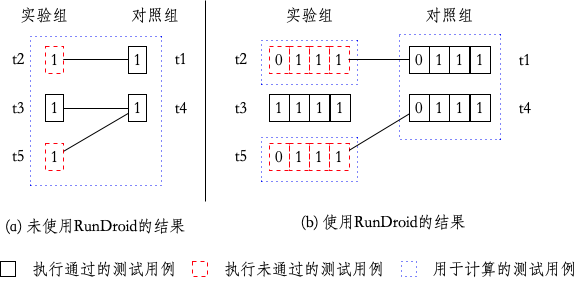
\includegraphics[width=0.8\textwidth]{./Figures/treatment.png}
	\end{center}
	\caption{使用RunDroid前后关于语句\Line{13}的测试用例匹配的对比}
	\label{fig:motivationResultTreatment}
\end{figure}

在$\tau$的结果中,分数最高包括\Line{4}、\Line{7}和\Line{13},均为0.67;
%在$\tau'$的结果中,分数最高只有\Line{13},分数从0.67提升到1。
而对于其他行,分数保持不变。
从结果上看,$\tau'$的结果比结果$\tau$更好。
理由是,在RunDroid接入后,错误语句的分数有所提高,同时错误语句与非错误语句得到区分。
\Line{13} 分数提高的原因如下:
在接入RunDroid前,方法\code{onClick(View)}和\code{TaskThread.run()}没有任何调用关系。
因此,\Line{13}的前驱节点集合中只包括控制依赖语句\Line{12} ,实验组和对照组的\code{Mdata(\Line{13})}数据如\autoref{fig:motivationResultTreatment}-(a)所示,所有的测试用例参与计算:$\tau= \frac{1+1+0	}{3} - \frac{0+0}{2} = 0.67$。
而接入RunDroid后,方法\code{onClick(View)}和\code{TaskThread.run()}产生关联(即触发关系),
%方法\code{onClick(View)}中\code{TaskThread.run()}
进而形成数据依赖关系。
\Line{13}的前驱节点增加了\Line{2}、\Line{5}和\Line{9},实验组和对照组的\code{Mdata(\Line{13})}如\autoref{fig:motivationResultTreatment}-(b)所示。
实验组中的测试用例$t_3$在对照组中找不到对应的测试用例,因此不参与计算。
最后,根据测试用例$t_1$、$t_2$、$t_4$、$t_5$得到\Line{13}的错误估计值:$\tau =  \frac{1+1	}{2} - \frac{0+0}{2} = 1$。
对于其他语句,前驱节点的信息并没有发生变化,因此数值保持不变。



\eat{

在\autoref{tab:result}中,我们在第13行显示了一个错误的语句示例。
而是直接传递,如果在传入方法之前它是一个正值,则应检查第13行的方法loadData(int)的参数。
第一列显示了与每个语句关联的行号的程序假设我们使用因果影响模型计算程序的失效原因,我们能够计算列“结果”中显示的估计数。第4,9和13行都是估计的,得分最高为0.67。
}
\eat{
	
	In Table 1, we show an example faulty program with a faulty statement at Line 13. 
	Instead being passed directly, the parameter of method loadData(int) at Line 13 should be checked if it is a positive value before passing into the method. 
	The first column shows the program with line numbers associated with each of its statements.
	Columns 2 through 6 represent test cases t1-t5, respectively. 
	The header of each test case column shows the values of v and num that are used at Lines 1 and 2, respectively. 
	The values for a test case column indicate whether the corresponding program statement is exercised by the test case, 1 for covered and 0 for not covered. 
	The bottom row shows the outcome of each test case execution, with “1” indicating a failing execution and “0” indicating a passing one.
	Suppose we compute the failure-causing effect of the program using the causal influence model [7, 8], we are able to compute the estimate numbers shown in Column “result”. Lines 4, 9, and 13 are all estimated with the highest score 0.67.
}



\eat{
因果影响模型以及许多其他故障定位技术考虑了动态程序依赖的影响,因为依赖信息不仅有助于触发故障的影响,而且还将它们传播到程序输出。
不幸的是,由于Android的特定编程范例,在显示的示例中无法捕获第8行和第11行之间的控制依赖性。
并且,丢失适当的控制流导致计算报告具有相同最高分的三个语句,从而使得故障定位技术在Android中不那么有效。
因此,为了改进Android应用程序的故障定位技术,RunDroid旨在通过运行时信息和执行期间的动态调用图来恢复非常需要的控制流依赖性。

}

\eat{



我们将激励性的例子作为主题计划。
因果影响模型在很大程度上依赖于陈述之间的依赖关系。
使用RunDroid,捕获了第9行\code{t.start()}和第11行\code{TaskThread.run()}之间的异步触发关系,因此第13行的前导是行$ \{ $ 5,8,9,13 $ \} $,而不仅仅是第13行,这是原始因果影响模型的情况。
\autoref {fig:motivationResultTreatment}显示治疗单位和控制单位及其相关的第13行测试用例。
具体来说,\autoref {fig:motivationResultTreatment} - (a)代表没有RunDroid的情况,而\autoref {fig:motivationResultTreatment} - (b)代表RunDroid的情况。
治疗单位是第13行的测试用例,分别为$ t_2 $,$ t_3 $和$ t_5 $;控制单元是不包括第13行的测试用例,是$ t_1 $和$ t_4 $。
对于目标语句,我们使用协变量向量在测试用例中显示其前任语句的封面信息。
显示了由测试用例生成的协变量值的向量。
在\autoref {fig:motivationResultTreatment} - (b)中,向量$ \langle $ 0,1,1,1 $ \rangle $表示对于测试用例$ t_2 $,只包含第5行,其他三个前任语句(第8,9,12行)都包括在内。
使用来自因果推理模型的相同方程,后一种情况的因果效应估计(来自RunDroid的依赖信息)的结果不同。
第13行的估计是$ \frac {(1 + 1)} {2} - \frac {(0 + 0)} {2} = 1.0 $。其他陈述的估计数见最右列表2。


}
	\eat{
		
		We take the motivating example as the subject program.
		Causal influence model relies heavily on dependence relationship among statements.
		With RunDroid, the asynchronized trigger relation between Line 9 \textit{t.start()} and Line 11 \textit{TaskThread.run()}, is captured, hence the predecessors of Line 13 are Lines ${\{}$5, 8, 9, 13$\}$, instead of Line 13 only, which is the case of original causal influence model.
		\autoref{fig:motivationResultTreatment} shows the treatment units and the control units with their associated test cases for Line 13.
		Specifically, \autoref{fig:motivationResultTreatment}-(a) represents the case of without RunDroid, and \autoref{fig:motivationResultTreatment}-(b) represents the case with RunDroid.
		The treatment units, which are test cases that cover Line 13 are $t_2$, $t_3$, and $t_5$; the control units, which are test cases that do not cover Line 13 are $t_1$ and $t_4$.
		For target statement, we use the vector of covariate to present the cover information of its predecessor statements in a test case.
		The vector of covariate values generated by the test cases is shown.
		In \autoref{fig:motivationResultTreatment}-(b), the vector $\langle$0,1,1,1$\rangle$ means that for test case $t_2$, only Line 5 is not covered, the other three predecessor statements (Lines 8, 9, 12) are all covered.
		Using the same equation from causal inference model, the causal-effect estimates for the latter case (with dependence information from RunDroid) are resulted differently. 
		The estimate for Line 13 is $\frac{(1+1)}{2}-\frac{(0+0)}{2} = 1.0$. The estimates for the other statements are shown in Table 2, in the far right column.
		
	}
	
	



\section{本章总结}
	


% 本章中,我们将环绕着构建效率、日志效率、运行效率等三个方面对RunDroid角进行系统性能测试和评估,并结合实验结果阐述了采用源代码插桩、基于MMap的日志方案等原因。

本章结合具体的使用场景对RunDroid生成的拓展函数调用图做了较为详细的描述。
同时,我们还对比分析在相同场景下静态分析工具FlowDroid的运行结果。
我们发现,RunDroid生成的调用图的完整性依赖于源代码处理以及待拦截的目标系统方法列表的完整程度,而FlowDroid的分析对象是Android应用程序APK文件,调用图的完整性受到自身算法实现的限制。
另外,两者在设计思想上不同的,RunDroid关心的是在程序执行过程中的方法之间的依赖关系,而FlowDroid反映的是从函数执行角度两个方法(包括递归调用)之间是否存在调用的可能性。
前者是某一应用运行的具体、微观的表现,而后者更多的是反映方法调用关系在宏观、理论上的可能性。
综上,RunDroid和FlowDroid体现方法的调用关系上各有千秋。

同时,我们将RunDroid和错误定位技术结合,进行了尝试性的实验。
实验结果显示,RunDroid生成的调用图中的方法触发关系可以将异步方法调用(例如Java 多线程和Handler)关联起来,补全函数间的控制依赖和数据依赖关系。
在RunDroid提供的信息的帮助下,基于因果模型的错误定位技术相关实验结果得到一定的提升,提高了实验结果的准确度。